\subsection{Modelado del problema}
El modelado del problema es una de los campos con mayor potencial dentro del FJSP, trabajar sobre una 
propuesta solida puede repercutirá directamente en el resultado final, por lo que es necesario
contemplar diferentes alternativas. En este apartado se desarrollará la propuesta final exclusivamente,
pero se hará referencia a otras alternativas que se han descartado dentro de la sección de "Posibles
representaciones del problema".

\subsubsection{Procedimiento para definir un environment de RL}
El RL es un tipo de aprendizaje automático que se basa en la interacción de un agente con el environment. 
Este agente toma decisiones en función de la información que recibe del estado y es recompensado 
o penalizado acorde a las decisiones que toma y su objetivo es maximizar la recompensa total o return
obtenida a lo largo del tiempo. Este tipo de técnicas se pueden utilizar para resolver problemas de optimización 
combinatoria en los que el espacio de estados es muy grande y no es posible explorar todas sus combinaciones. 
En casos en los que el espacio de estado del problema es muy grande o cambia continuamente,
el aprendizaje por refuerzo puede ser útil para encontrar soluciones óptimas sin necesidad de
explorar todo el espacio de estado. Podemos definir un environment de RL formalmente de la siguiente manera:

\begin{itemize}
    \item \textbf{Espacio de estados (S):} Es el conjunto de todos los posibles estados del environment. 
    Puede ser finito o infinito, y se denota como $S = \{s1, s2, ..., sn\}$, donde si S es finito, n representa 
    el número de estados posibles. Por ejemplo, si estuviéramos modelando un juego de ajedrez, el espacio 
    de estados incluiria todas las posibles configuraciones del tablero.

    \item \textbf{Espacio de acciones (A):} Es el conjunto de todas las posibles acciones que un agente 
    puede tomar en el environment. Al igual que el espacio de estados, el espacio de acciones puede ser finito 
    o infinito, y se denota como $A = \{a1, a2, ..., am\}$, donde si es finito, m representa el número de 
    acciones posibles. Siguiendo con el ejemplo del juego de ajedrez, el espacio de acciones podría incluir 
    todos los posibles movimientos que un jugador puede hacer en su turno.

    \item \textbf{Función de transición de estados (T):} Es una función que define la probabilidad de transición 
    de un estado a otro estado dado una acción tomada por el agente. Se denota como T(s, a, s'), donde s es el 
    estado actual, a es la acción tomada y s' es el siguiente estado alcanzado después de tomar la acción a en 
    el estado s. Formalmente, la función de transición se puede escribir como: T: S x A x S -> [0, 1], donde 
    [0, 1] representa el rango de probabilidades.

    \item \textbf{Función de recompensa (R):} Es una función que asigna una recompensa numérica a una transición 
    de estado y acción específica. Se denota como $R(s, a, s')$, donde s es el estado actual, a es la acción tomada, 
    s' es el siguiente estado alcanzado después de tomar la acción a en el estado s, y $R(s, a, s')$ es 
    la recompensa asociada a esa transición. Formalmente, la función de recompensa se puede escribir 
    como: $R: S x A x S -> R$, donde R es un valor numérico que representa la recompensa. 
\end{itemize}

\textbf{Nota: } En nuestro caso, no será necesario definir una función de recompensa, ya que debido a la 
naturaleza del Imitation Learning no requiere de una función de recompensa. Esto se debe a que el agente 
no toma decisiones por si mismo, sino que aprende a tomar decisiones a partir de un experto.

\subsubsection{Representación del estado}
\paragraph{Grafos heterogéneos}
La propuesta del estado se basa en una representación mediante el uso de un grafo heterogéneo. Un grafo 
heterogéneo es un tipo de grafo en el que los nodos y/o aristas pueden tener diferentes tipos, atributos 
y propiedades. Esto significa que se pueden representar diferentes relaciones, y pueden tener distintas 
características asociadas a ellas. Por ejemplo, en un caso donde se quiera modelar una red social, 
los nodos podrian representar personas, contenidos o grupos y las aristas amistades, seguidores, 
miembros de un grupo, etc.\medskip 

En el caso del FJSP es posible representar las operaciones, máquinas y trabajos como nodos del grafo, 
y a su vez las aristas se pueden utilizan para asignar las restricciones del problema, como los tiempos de 
procesamiento, las dependencias entre tareas y la asignación de las mismas. Esto permite una representación 
compacta de la información relevante del problema, siendo una de sus virtudes que, a medida que se aumenta 
el número de máquinas y operaciones, simplemente se agregarán más nodos y aristas al grafo, lo que no 
implicara un aumento exponencial en la complejidad de la representación, permitiendo asi una escalabilidad 
natural en términos de la representacion del problema. Otra de sus ventajas es que las operaciones sobre 
grafos, como la búsqueda o manipulación de nodos y aristas, son operaciones computacionalmente eficientes. 
Esto permite realizar cálculos y análisis en tiempo razonable, incluso cuando el tamaño del problema incrementa. 

\begin{figure}[ht]
    \centering
    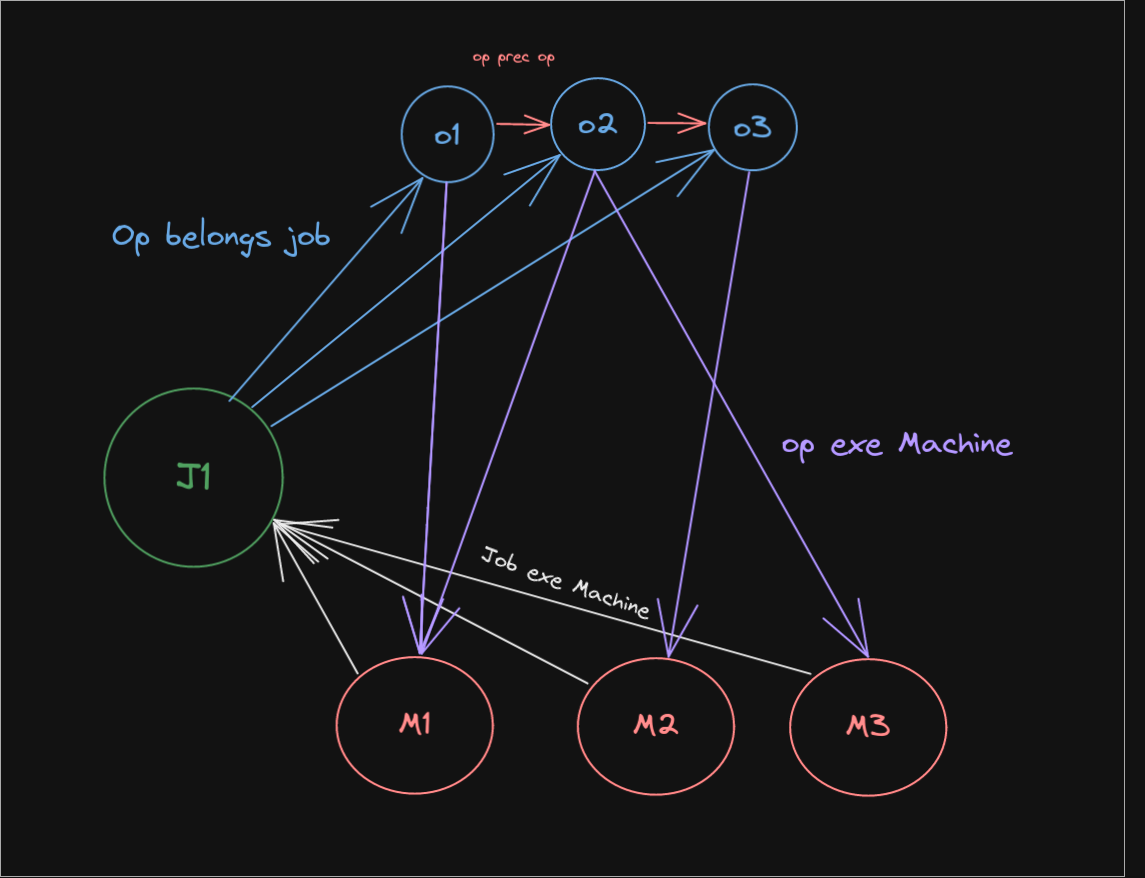
\includegraphics[scale=0.34]{graphv1.png}
    \caption{Ejemplo simplificado de un grafo heterogéneo para el FJSP}
    \label{fig:grafo-heterogeneo}
\end{figure}

Como se puede ver en la Figura \ref{fig:grafo-heterogeneo}, hemos representado mediante un grafo
heterogéneo una instancia del FJSP que cuenta con 3 máquinas, 1 trabajo y 3 operaciones. En este caso, 
la operación 1 solo puede ser ejecutada en la máquina 1 y es por ello que no está conectada con 
las otras máquinas mediante la relación `Operacion Ejecuta Maquina'. Aclarar que por motivos de 
simplifición, no se han incluido todos los diferentes tipos de relaciones existentes entre 
los nodos y solo están representadas las relaciones más importantes. Se debe tomar como una ayuda 
visual para entender el potencial que tiene este tipo de representaciones, durante las siguientes 
secciones detallaremos en profundidad todas las características de los nodos y de sus relaciones.

\paragraph{Tipos de nodos y sus características}
\begin{itemize}
    \item \textbf{Operación (O):} La operación es la unidad fundamental de trabajo en el FJSP. Cada 
    operación tiene un identificador único, un flag que indica si ha sido ejecutada,
    un flag que indica si es posible ejecutar la operación y el número de máquinas en las que puede
    ser ejecutada.
    \item \textbf{Trabajo (J):} Representa un conjunto de operaciones que deben ser ejecutadas 
    en una secuencia determinada. Cada trabajo tiene un identificador único, el tiempo de 
    procesamiento de la ultima operación, el numero de operaciones restantes y el gap total
    existente entre todas las operaciones del job.
    \item \textbf{Máquina (M):} Representa una máquina dentro del problema del FJSP. Cada máquina 
    cuenta con un identificador único, el tiempo de procesamiento acumulado de todas sus operaciones,
    el gap total existente entre todas las operaciones de la máquina y la diferencia entre el tiempo
    de procesamiento entre ella y la máquina con menor tiempo de procesamiento.  
\end{itemize}

\paragraph{Tipos de relaciones entre nodos}
\begin{itemize}
    \item \textbf{Operación - precede - Operación:} Esta relación indica que la operación 1 debe ser
    ejecutada antes que la operación 2. Se utiliza para representar las dependencias entre operaciones
    dentro de un mismo trabajo.
    \item \textbf{Operación - pertenece - Trabajo:} Esta relación indica que la operación 1 pertenece
    al trabajo 1. Se utiliza para representar las dependencias entre operaciones y trabajos.
    \item \textbf{Trabajo - escucha - Trabajo:} Relación auxiliar que se utiliza para conectar los
    nodos de trabajo y proveer de información a los nodos de la red.
    \item \textbf{Trabajo - escucha - Máquina:} Relación auxiliar que se utiliza para conectar los
    nodos de trabajo con los nodos y máquina para proveer de información a los nodos de la red.
    \item \textbf{Máquina - escucha - Trabajo:} Similar a la relación anterior, pero en este caso
    las relaciones se establecen en sentido opuesto.
    \item \textbf{Operación - exec - Máquina:} Relación entre las operaciones y las máquinas que indica
    que la operación 1 puede ser ejecutada en la máquina 1. Esta relación cuenta con un atributo que
    indica el tiempo de procesamiento de la operación 1 en la máquina 1.
    \item \textbf{Máquina - ejecuta - Trabajo}: Relación directa entre la máquina y el trabajo, esta
    relación indica que la máquina 1 ejecuta el trabajo 1. Adicionalmente, esta relación cuenta con
    un atributo que indica el tiempo de procesamiento de la operación que se está ejecutando en el
    trabajo 1 para la máquina 1.
    \item \textbf{Máquina - gap - Trabajo}: Misma relación que la anterior, pero esta intercambia el
    atributo de tiempo de procesamiento por el gap que generaría la operación que se está ejecutando
    en el trabajo 1 si se llegase a aplicar en la máquina 1.
\end{itemize}

\paragraph{Representación final}
Para finalizar, se muestra la representación que tendria un estado tomando en consideracion el ejemplo 
de la Figura \ref{fig:example-solution} utilizada en la introducción. En la siguiente figura ahora ya 
se pueden apreciar todas las relaciones mencionadas con anterioridad, y para conocer en mayor profundidad
como se ha implementado puede consultar la sección de desarrollo. Hemos querido continuar con el ejemplo
que se ha utilizado en la introducción y en el resto de la seccion tambien se hará referencia a este
para ilustrar las futuras explicaciones. 

\begin{figure}[ht]
    \centering
    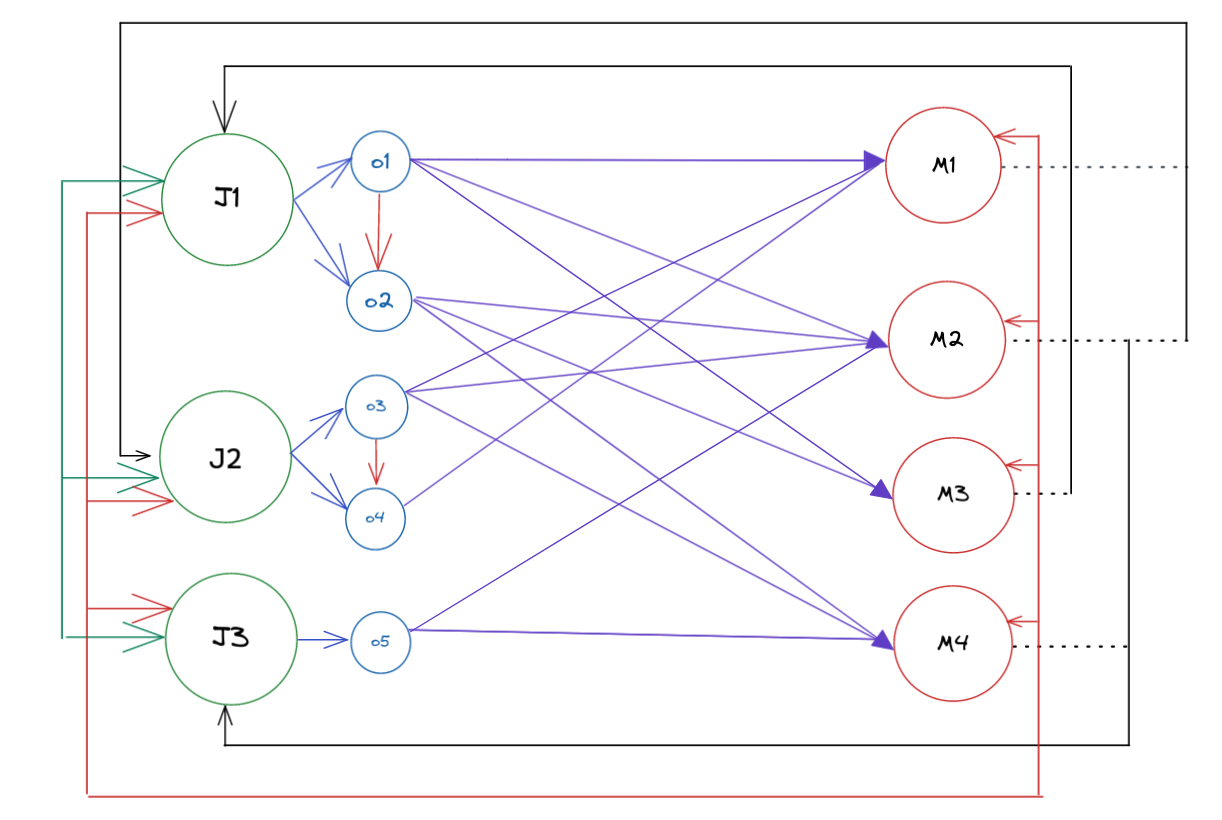
\includegraphics[scale=0.33]{final.png}
    \caption{Estado inicial del la instancia presente en el Cuador 1}
    \label{fig:final-solution}
\end{figure}

% La justificación de usar PyTorch Geometrics es que ofrece soporte para el procesamiento de grafos,
% lo que significa que se puede utilizar para trabajar con redes de datos en las que los nodos están
% conectados por enlaces. Esto puede ser útil porque mediante técnicas de Deep Learning se puede analizar
% la estructura y las relaciones que existen entre los nodos de un grafo. Además, la librería ofrece herramientas
% para trabajar con diferentes tipos de grafos, como grafos dirigidos y heterogéneos, que son los utilizados en
% nuestra representación, y proporciona una serie de funciones para realizar operaciones básicas con grafos.

\subsubsection{Espacio de acciones}
El espacio de acciones es el conjunto de acciones que puede realizar el agente en cada estado. 
En nuestro caso, se pueden definir el conjunto de acciones como la lista de todas las tuplas 
formadas por las operaciones que pueden ser ejecutadas en cada estado y las máquinas en las que
pueden ser ejecutadas. Por ejemplo, en el estado de la Figura \ref{fig:final-solution} se pueden
definir las siguientes acciones: (Maquina 1, Operacion 1), (Maquina 1, Operacion 3), 
(Maquina 2, Operacion 1), (Maquina 2, Operacion 3), (Maquina 2, Operacion 3), (Maquina 3, Operacion 1), 
(Maquina 4, Operacion 5). En este caso, todas aquellas operaciones que no se encuentren en la lista 
de acciones disponibles no pueden ser ejecutadas en el estado actual.

\subsubsection{Transición de estados}

\pagebreak
